\subsection{Checklists}
Much of this data is repeated in more detail later in the document,
which should be read before use (at least up to and including section~\ref{angcont}).
\subsection{Rover startup checklist}
\begin{enumerate}
\item Ensure the battery inside the main compartment is charged.
\item Ensure main compartment lid is closed.
\item Switch on PCs using the PC power button.
\item If it's installed, you may wish to switch off the science PC (the right-hand PC). The button is on
the front of the PC, near the floor of the compartment.
\item Check current is less than 2A.
\item Connect a laptop to the rover's WiFi network (the SSID contains ``EnGenius'').
\item SSH into the rover: host 192.168.0.10, username \emph{blodwen}, password \emph{robotics}.
\item Switch on the motors with the other power switch on the lid.
\item Check that the underside lights go steady on, then flash at about 1Hz.
\item Check current is about 1.8 to 2A.
\item (The list from here implies direct rover control via Angort)
\item In the terminal SSHing into the rover, issue the commands
\begin{v}
cd r
./rover
\end{v}
\item Ensure the connection is made --- \texttt{READY} should appear
and the Angort prompt \texttt{1|0>}.
\item Issue the commands
\begin{v}
reset calib
\end{v}
to reset the initial boot exception state and send calibration data.
\item Now refer to section~\ref{angcont} for commands.
\item In the case of an emergency, hammer CTRL-D (or CTRL-C if that
fails) to send an emergency stop. All gains will be zeroed, and 
\texttt{reset calib} must be reissued to restart the rover.
\end{enumerate}
\subsection{Rover shutdown checklist}
\begin{enumerate}
\item Exit the Angort interpreter with CTRL-D or \texttt{quit}.
\item Switch off the motors.
\item Power down the locomotion PC with \texttt{sudo poweroff}.
\item Wait for the power consumption to drop to about 1A (indicating
PC powerdown).
\item Switch off the PC power using the other power switch.
\end{enumerate}



\section{Introduction}
The rover's control architecture consists of three layers, as shown
in figure~\ref{fig1}:
\begin{description}
\item[A PC running the main control software] which is interfaced to the
hardware via a register interface. It sends register read/write commands
to the Arduino. In many situations, this control layer will itself
be a server responding to commands sent by another system.
\item[An Arduino accepting register read/write commands] which passes
them over
\isqc{} to nine motor controllers. This is referred to in the text as
the \textbf{master controller.} It also has a set of registers of its own
for global system information.
\item[Nine motor controller boards]\footnote{Sparkfun ``serial controlled
motor driver'' boards, ROB-09571} each containing an ATMega328p processor
(effectively an Arduino) to handle the PI control algorithms and respond
to register read/write commands for two motors, using an
L298P dual H-bridge to drive the motors. Each board may also have an analogue
input for the chassis potentiometer.

These are
referred to in the text as \textbf{slave} or \textbf{secondary controllers.} 
\end{description}

\begin{figure}[ht]
\center
\includegraphics[width=6in]{fig1.pdf}
\caption{Overall architecture}
\label{fig1}
\end{figure}

All software is written in C++, with the both master and slave controller
code being written in the Arduino variant, burned directly into the chip
using ICSP.

\subsection{Wheel pair architecture}
\label{whpairarc}
The rover has six wheels, each pair of which is controlled by three
slave controllers as shown in figure~\ref{fig2}.
This shows that there are two distinct kinds of slave controllers:


\begin{figure}[ht]
\center
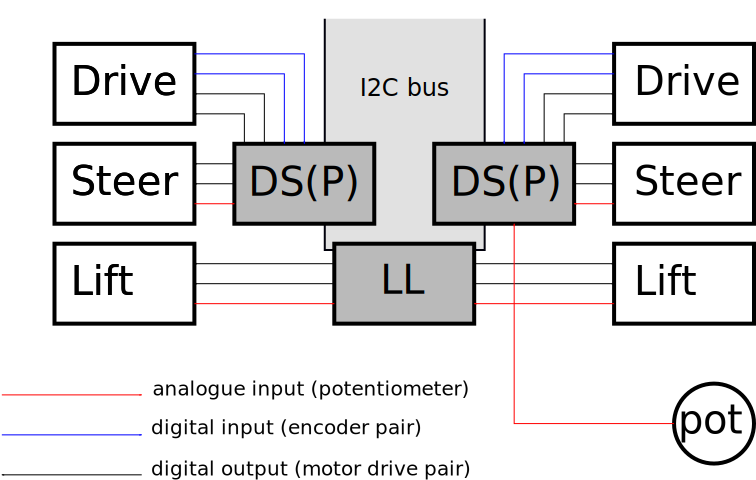
\includegraphics[width=4in]{hardwareoverview.pdf}
\caption{Hardware overview of a single wheel pair}
\label{fig2}
\end{figure}

\begin{description}
\item [Two Drive/Steer/(Position) controllers per pair,] which each control the driving
and steer motor on one wheel. One of these also receives an input from
one of the three chassis configuration potentiometers. On the other, this
input is ignored.
\item [One Lift/Lift controller per pair,] which control the lift motors on both wheels.
\end{description}
The reason for this split is that each controller board can only handle 
two analogue inputs (in addition to the two internal current sensor channels.)

The controllers and the wheels they control are numbered as in figure~\ref{fig3}.
The wheel numbering scheme is that given in the rover documentation.

\begin{figure}[ht]
\center
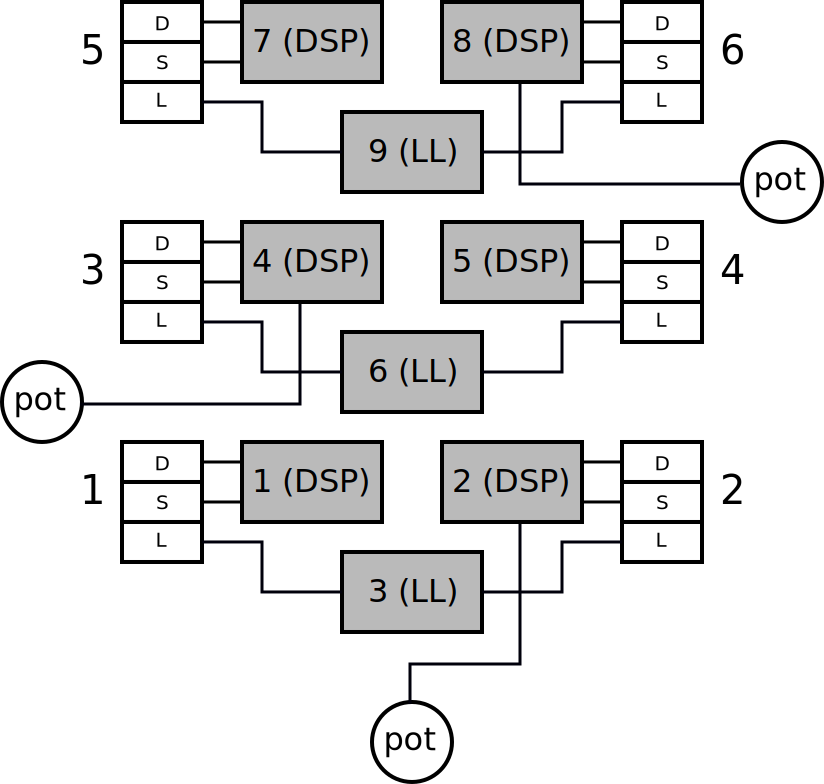
\includegraphics[width=4in]{numbering.pdf}
\caption{Numbering of controllers and wheels}
\label{fig3}
\end{figure}

\clearpage
\section{Using the rover}
The rover is shown in Figure~\ref{fig:blod}. 
\begin{figure}[ht]
\center
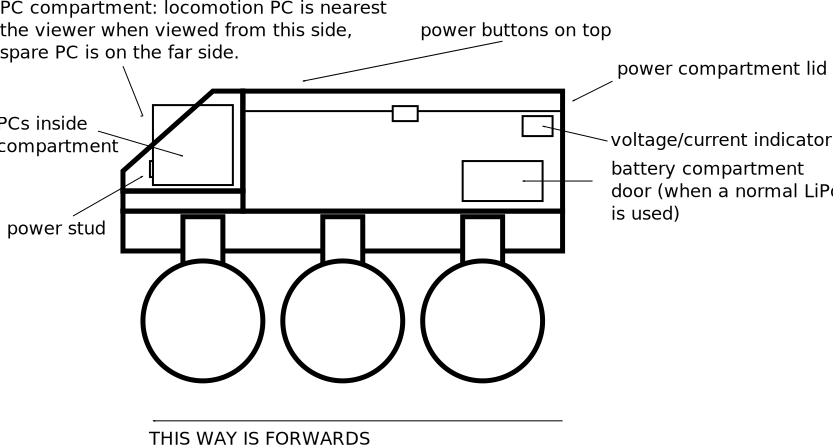
\includegraphics[width=5in]{blod.pdf}
\caption{The Blodwen rover}
\label{fig:blod}
\end{figure}
Note that the rover's ``front'' is the obvious, wedged end.


\begin{itemize}
\item The main compartment contains a LiPo battery suitable for most applications. Ensure this is charged
prior to use.
\item The battery compartment has space for an extra LiPo battery. If you are using this, the connector
needs to be passed through from the main compartment. Ensure you connect with the correct polarity.
\item Switch on the rover PCs by pressing the PC power button on the roof of the chassis.
\textbf{Once this has been done, do not power off the rover without shutting the locomotion PC down from
a terminal connection.}
\item Check that the voltage and current are nominal (11.5-12V, $<3$A) using the indicator. If they are
not, shut down the rover and power off.
\item The PCs are in the wedge-shaped compartment at the front of the rover.
If another PC is in use, switch off the spare PC. This is the PC located on the right side of the rover.
The power studs are located at the bottom of the PC
front panels. Figure~\ref{fig:blod2} shows the arrangement of the PCs more clearly. Power consumption should drop
to $\sim 1.5$A.
\begin{figure}[ht]
\center
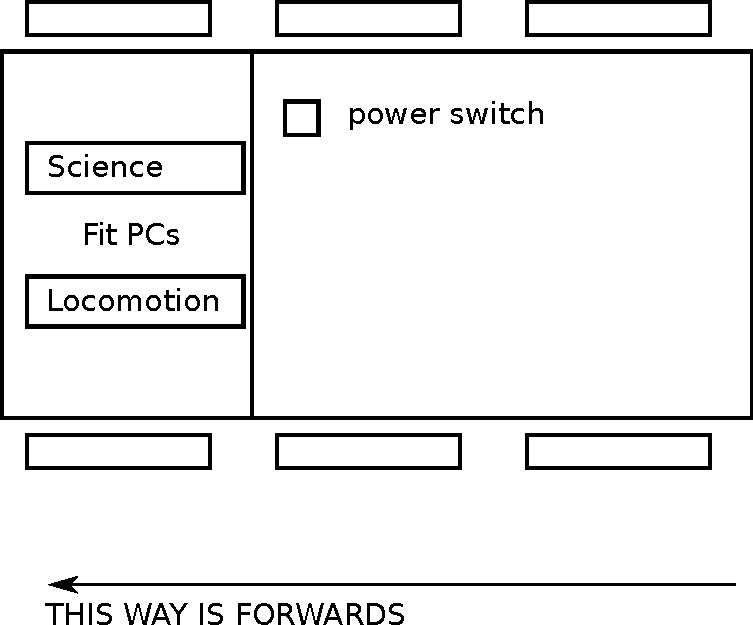
\includegraphics[width=3in]{blod2.pdf}
\caption{The Blodwen rover, from above}
\label{fig:blod2}
\end{figure}
\item To power up the motor, drive and chassis electronics the motor power switch on the lid should be pressed.
\item The lights under the chassis should come on briefly, and then begin to flash approximately
once a second. Power consumption should rise to $\sim 1.8-2$ A. The hardware is now ready to receive commands. Proceed to
section~\ref{angort} to find out how to command it with the Angort language.
\end{itemize}

\subsection{Detailed explanation of LED flashes}
This guide may help diagnose wiring problems inside the rover chassis:
\begin{itemize}
\item Each controller has two LEDs. As the rover boots, each controller
should show the lowest 2 bits of its \isqc{} address (1-9) on the LEDs
for about half a second. This causes the initial lighting state.
\item The master and slaves will start in the boot exception state,
so the LEDs will be steady on. Shortly after boot, the master will attempt to send
resets to each slave. 
\item If the send fails, the \isqc{} bus will hang, so the master's
watchdog timer will time out and the master will reboot and try again. A
common failure mode is repeated reboot cycles, where the the good slaves
are resetting successfully from the boot exception, shown by repeated off
gaps, while the bad slave will just show a steady exception state (see
below).
\item If the slaves all reset successfully, the master will receive
the acknowledgements and begin awaiting PC packets. It will also
send a ``ping'' message to the slaves once per second. If a slave receives
this, it will briefly flash an LED (LED1 on a drive/steer unit,
LED2 on a lift/lift unit). Therefore, the LEDs should flicker once per
second on all slaves once the rover is ready to receive commands.
\end{itemize}

In the exception state, the two LEDs will stay on showing:
\begin{itemize}
\item LED1: motor 1 is in exception
\item LED2: motor 2 is in exception
\item both LEDs: the exception is not a motor exception
\end{itemize}

\subsubsection{Using the remote control}
\textbf{(Note: this hasn't been tested for a while).}
Turning on the remote control causes the master's main loop to ignore any
instructions sent from the PC, and also recalibrates the rover (i.e. a new
set of PID and extent parameters will be sent). Therefore, the rover will
need to be recalibrated (by calling the \textbf{calibrate()} method) if
PC control is desired again.

When the remote control is active, a blue LED should shine under the rover,
clearly visible on the driving surface. The controls are as follows:
\begin{itemize}
\item Left stick forward/backward : drive speed
\item Right stick left/right: turn steer wheels
\item Right stick forward: alternate steer mode
\end{itemize}
By default, steering operates using Ackermann steering on the front
and back wheel pairs in opposite directions, with the centre wheels not commanded.
If the right stick is pushed forwards to its limit, the same steering angle
will be applied to all wheels, permitting ``crabbing''.

\subsection{Controlling the rover with Angort}
\label{angort}
The rover locomotion PC has the language Angort installed, with a set of scripts and native C++ word
definitions to allow easy control. To run the language interpreter, one must connect to the locomotion
PC via SSH. Both PCs are connected to a WiFi router installed inside the rover.

\subsubsection{Connecting to the rover and starting Angort}
\begin{itemize}
\item Power up the rover. Power down the science/spare PC immediately (see above).
\item Connect to the rover on the EnGenius router via SSH (IP address 192.168.0.10, username
\textbf{blodwen}, password \textbf{robotics}).
\item \texttt{cd r} to get into the appropriate directory (this is a soft link to a subdirectory).
\item Power on the electronics by closing the battery door.
\item \texttt{./rover} to start a special version of the Angort interpreter with rover control words
added. The script \texttt{script.ang} will automatically
be loaded --- it contains a useful set of word definitions to enhance those built in.
\item A few lines should show the connection to the master Arduino being established, and initial rover library setup. 
The Angort prompt
\begin{v}
1|0 >
\end{v}
should appear (the left number is the number of GC-objects in the system, the right number is
the depth of the stack). If this initial connection phase fails, check that the safety switches are
closed and that the microcontrollers are all flashing as they should.
\end{itemize}

\subsubsection{Rover control commands}
\label{angcont}
The rover boots in an exception state as a safety feature, and also has all PID gains in the motors
set to zero. Before it can move, all the controllers need to have their exceptions reset, and correct
PID gains uploaded. To do this, issue the following commands \textbf{but be prepared to hammer CTRL-D}:
\begin{v}
reset calib
\end{v}
This may result in some small motion of the wheels if the rover has been moved by hand or is
in an unusual configuration for some other reason. \textbf{If the motion is dangerous, hit CTRL-D} to
reset the system.

Once this has been done, movement commands may be issued. If they appear to do nothing, check
that \texttt{reset} and \texttt{calib} have been run.
The following table shows examples of the most common commands for controlling the rover:

\begin{tabular}{|l|p{4in}|} \hline  
\texttt{1000 d} & \textbf{set all drive motors to speed 1000} forwards, towards the wedged end with the PCs.\\
\texttt{-2500 d} & \textbf{set all drive motors to speed -2500}, i.e. backwards --- note that 2500 is about the highest safe speed.\\
\texttt{40 t} & \textbf{turn $40^\circ$,} done by setting the front steer wheels to the given angle and the rear wheels to
the opposite.\\
\texttt{-40 t} & \textbf{turn the opposite way} to the previous command.\\
\texttt{40 a} & \textbf{set all steer motors to $40^\circ$,} useful for ``crabbing''.\\
\texttt{20 setliftall} & \textbf{set all lift motors} to $20^\circ$.\\
\texttt{20 1!lift} & \textbf{set lift lift motor 1} to $20^\circ$. The notation
\begin{v}
<value> <motornumber>!<motortype>
\end{v}
can be used to set individual drive, steer and lift motor speeds and positions. \textbf{Be careful} ---
it's possible to make the rover perform potentially damaging actions by setting individual motors.\\
\texttt{1?lift.} & \textbf{get and print the requested position for lift motor 1.}
\\ \hline
\end{tabular}

\subsection{Monitoring the rover graphically}
The Angort scripting system, once connected to the rover hardware, constantly sends a stream of key/value
pairs over UDP to port 13231 on host 192.168.0.100 (the first router address available to WiFi hosts). 
The \texttt{monitor} program can read this data and display it graphically with an appropriate configuration
file.

The program is available at \url{https://github.com/jimfinnis/monitor.git} and is a Qt4 application. It
requires the \texttt{libmarblewidget} library to compile (adding support for mapping; the monitor
is also used for robotic boat trials). A suitable configuration file is provided --- once compiled, run
the program with
\begin{v}
monitor -f ./roverconfig
\end{v}
This configuration will display the desired and actual drive motor speeds, the actual lift and
steer positions, the current readings for the 6 drive wheel controllers, the temperatures of all
9 controllers above ambient. Extra variables are shown for hormone settings and traversed distance,
but these are provided by code built for particular experiments beyond the scope of this document.
